\documentclass{article}
\usepackage{graphicx} % Required for inserting images
\usepackage{tikz}
\usetikzlibrary{shapes.multipart}
\usetikzlibrary{arrows.meta}
\usepackage{hyperref}
\usepackage{minted}
\usepackage{xcolor}
\usepackage{ulem}
%\usepackage{pygments.lexers.yara}

\definecolor{codebackground}{rgb}{0.95,0.95,0.92}
\definecolor{shellbackground}{rgb}{0.2,0.2,0.1}
\definecolor{shelltext}{rgb}{1,1,1}
\definecolor{codekeyword}{rgb}{0.6,0,0.6}

\usemintedstyle{friendly}
\newminted[yaracode]{cpp}{
    bgcolor=codebackground,
    linenos,
    breaklines,
    frame=lines,
    framesep=2mm,
    rulecolor= \color{codekeyword},        
    framesep=3mm,
    fontsize=\small,

}

\title{ CSE 406 Presentation Report : Malware analysis by YARA }
\author{ \textsuperscript{1} Alina Zaman : 1905099 \\
\textsuperscript{2} Saha Kuljit Shantanu : 1905119}

\date{March 9, 2024}

\begin{document}

\maketitle

\section{ Introduction }

\textbf{YARA} is a powerful tool that has been fascinating malware analysts. The purpose of YARA encompasses the detection of presence of evil in malware by pattern or string matching. After complete analysis, the malware can be classified using the YARA tool.

\section{ Getting Started }



The installation of YARA in Ubuntu Linux is quiet a short and convenient process. Here it is step by step
\begin{itemize}

\item Navigating to \href{https://yara.readthedocs.io/en/stable/gettingstarted.html}{\textcolor{cyan}{\uline{this link}}}, the first instruction we get is to install the source code tarball file from \href{https://github.com/VirusTotal/yara/releases}{\textcolor{cyan}{\uline{https://github.com/VirusTotal/yara/releases}}}. The latest version is \textbf{4.5.0}

\item Now that the source-code.tar.gz is installed, it is time to compile it, hence we run the following commands in order, to unzip :

\begin{minted}[bgcolor= shellbackground, formatcom= \color{shelltext}]{bash}

$ tar -zxf yara-4.5.0.tar.gz
$ cd yara-4.5.0

\end{minted}

\item Now we have to install all the dependencies before compilation :


\begin{minted}[bgcolor= shellbackground, formatcom= \color{shelltext}]{bash}

$ sudo apt-get install automake libtool make gcc pkg-config
$ sudo apt-get install flex bison

\end{minted}

\item Now it is time to start the compilation of YARA tool :


\begin{minted}[bgcolor= shellbackground, formatcom= \color{shelltext}]{bash}

$ ./bootstrap.sh

\end{minted}

\item Now it is necessary to install the openSSL library and configure the tool as the tool cannot be configured without openSSL library :


\begin{minted}[bgcolor= shellbackground, formatcom= \color{shelltext}]{bash}

$ sudo apt-get install libssl-dev
$ ./configure
$ make
$ sudo make install

\end{minted}

\item Now that the tool is compiled and configured, we have to test if all packages are installed


\begin{minted}[bgcolor= shellbackground, formatcom= \color{shelltext}]{bash}

$ make check

\end{minted}

\item Now we need to test the tool by executing our yara rule :


\begin{minted}[bgcolor= shellbackground, formatcom= \color{shelltext}]{bash}

$ yara <yara-rule-file> <test-file-or-folder>

\end{minted}

If yara-rule is executed on a folder, it executes the rule for all file inside the directory recursively

To print elaborately on every line of every file where the rules match on the conditions :

\begin{minted}[bgcolor= shellbackground, formatcom= \color{shelltext}]{bash}

$ yara -s -r <yara-rule-file> <test-file-or-folder>

\end{minted}

\end{itemize}

\section{ Opening Malware }

The malware we were supplied for analysis by YARA tool was "libxselinux.so" which is a library file that has powerful properties to make system calls when any other c program includes it and executes itself.\\
\\
Executing the malware in local machine is a risk factor, hence it is not feasible to execute the file. However, the malware can be opened in hexadecimal format and assembly format.\\
\\
We can open the malware "libxselinux.so" into some file "libxselinux.txt" in hexadecimal format through the following command:

\begin{minted}[bgcolor= shellbackground, formatcom= \color{shelltext}]{bash}

    $ xxd libxselinux.so > libxselinux.txt
    
\end{minted}
We can open the malware "libxselinux.so" into some file "libxselinux.asm" in x86 assembly encoding format through the following command:

\begin{minted}[bgcolor= shellbackground, formatcom= \color{shelltext}]{bash}

    $ objdump -d -S libxselinux.so > libxselinux.asm
    
\end{minted}

\section{ Identifying the file type of malware }

In YARA, we can easily identify a file by a hidden specific property in the hex file. If the file is an \textbf{exe} file, it will have identifying tokens 'MZ' at the starting of the file :



\begin{yaracode}

rule test_IS_EXE_FILE {

    meta : 

        description = "Let's see if the file is exe"
        author = "Saha Kuljit Shantanu"
        date = "05-03-2024"

    strings :

        $exe_sign = { 4D 5A } //contains MZ

    
    condition: 

        $exe_sign at 0

}

\end{yaracode}
If the file is an \textbf{exe} file, it will have identifying tokens 'ELF' following any character at the starting of the file :

\begin{yaracode}

rule test_IS_OUT_FILE {

    meta : 

        description = "Let's see if the file is out file"
        author = "Saha Kuljit Shantanu"
        date = "05-03-2024"

    strings :

        $out_sign = { ?? 45 4C 46 } //contains .ELF

    
    condition: 

        $out_sign at 0

}

\end{yaracode}
We can also verify if the file is a deb file by the following rule:

\begin{yaracode}
    
rule test_IS_DEB_FILE {

    meta : 

        description = "Let's see if the file is deb file"
        author = "Saha Kuljit Shantanu"
        date = "05-03-2024"

    strings :

        $deb_sign = { 21 3C 61 72 63 68 3E } 

    
    condition: 

        $deb_sign at 0

}

\end{yaracode}
The malware may be a zip file with an outfile inside it, that executes on unzipping. For verification we check the following rule :

\begin{yaracode}
    
rule test_IS_OUT_FILE_IN_ZIP {

    meta : 

        description = "Let's see if the file is safe to unzip"
        author = "Saha Kuljit Shantanu"
        date = "05-03-2024"

    strings :

        $zip_sign = "PK\x03\x04" 
        $out_sign = ".out"

    
    condition: 

        $zip_sign at 0 and any of them

}

\end{yaracode}
When this property is tested on our malware, we get the output as in the figure \\

\begin{figure}[!h]

    \centering
    \includegraphics[width=\textwidth]{file_ver.jpg}
    \caption{Classifying the file of malware}
    \label{fig:file_type}
    
\end{figure}






\section{ Matching pattern to detect evil on malware }

\subsection{ Matching regular string }

By the following string matching rule, we can manually track the presence of keywords \textbf{NOP}, \textbf{GNU} or \textbf{SOCKET} in the malware to estimate if the malware fills the memory with NOPs, or compiles a c code or, opens a socket connection respectively : \\ \\

\begin{yaracode}

//Normal string matching

rule test_NOP_GNU_SOCKET { 

    meta : 

        description = "Let's see if the file has nops, or can compile with gnu or can open a socket"
        author = "Saha Kuljit Shantanu"
        date = "05-03-2024"

    strings :

        $nop = "NOP" nocase
        $gnu = "GNU" nocase
        $socket = "SOCKET" nocase

    
    condition: 

        $nop or $gnu or $socket
    
    
}

\end{yaracode}

\subsection{ Matching regular expressions }

By the following regular expression matching rule, we can manually track the malware to estimate whether it can take input from a program and give output to console : \\

\begin{yaracode}

//Matching with regular expressions

rule test_SCAN_PRINT { 

    meta : 

        description = "Let's see if the file has scanning and printing properties"
        author = "Saha Kuljit Shantanu"
        date = "05-03-2024"

    strings :

        
        $scan = /[a-z]{0,}scanf[a-z]{0,}/   
        $print = /[a-z]{0,}printf[a-z]{0,}/
        $get = /[a-z]{0,}get[a-z]{0,}/   
        $put = /[a-z]{0,}put[a-z]{0,}/

    
    condition: 

        $scan or $print or $get or $put
    
    
}


\end{yaracode}

\subsection{ Matching Hexadecimal pattern }

\begin{yaracode}

//Matching with hex strings

rule is_FILE_OUT {

    meta : 

        description = "Let's see if the file is an out file"
        author = "Saha Kuljit Shantanu"
        date = "05-03-2024"

    strings :

        $is_out = { ?? 45 4C 46 }

    condition:

        $is_out


}

\end{yaracode}

\section{ Checking conditions to analyse malware }

\subsection{ Detecting system calls }

By the following rule, we can detect if the malware is susceptible to make system calls : \\

\begin{yaracode}

//Detecting system call

rule is_CALLING_SYSTEM {

    meta : 

        description = "Let's see if the file is making system calls"
        author = "Saha Kuljit Shantanu"
        date = "05-03-2024"

    strings :

        $fclose = "fclose"
        $fopen = "fopen"
        $sleep = "sleep"

    condition:

        2 of them


}


\end{yaracode}

\subsection{ Detecting visibility of malware }

By the following rule, we can detect if the malware is susceptible to hide its existence : \\

\begin{yaracode}

//Matching malware invisibility

rule is_SELF_INVISIBLE {

    meta : 

        description = "Let's see if the malware is hiding itself"
        author = "Saha Kuljit Shantanu"
        date = "05-03-2024"

    strings :

        $eax = "_invisible" nocase

    condition:

        $eax


}


\end{yaracode}
The output to the evil detecting rules on our malware yields the following result \\

\begin{figure}[!h]

    \centering
    \includegraphics[width=\textwidth]{pt.jpeg}
    \caption{Detecting evil from the malware}
    \label{fig:file_evil}
    
\end{figure}

\section{Modules}

\subsection{PE and ELF}

The PE module includes a \textbf{is\_pe} variable that verifies whether the malware is an executable file. 
\\
\\
Moreover, the PE module includes both \textbf{DLL} and \textbf{characteristics} variables that verify whether the malware is a dynamic library file. As a matter of fact, every executable file links to a dynamic library, hence a dynamic library file may not be executable but an executable file is always dynamic link library.
\\
\\
The ELF module includes a \textbf{machine} variable that keeps the properties of machine code and assembly code of the malware and verifies whether the malware is an output file. In our case, the assembly is X86 and the machine code is 64-bit. Hence we choose to verify \textbf{EM\_X86\_64} which means output file with X86 assembly coding and 64-bit machine language.
\\
\\

\begin{yaracode}


import "pe"
import "elf"


rule elf_64
{
    condition:
        elf.machine==elf.EM_X86_64
}

rule is_dll
{
    condition:
        pe.characteristics & pe.DLL
}

rule is_pe
{
    condition:
        pe.is_pe
}


\end{yaracode}
The output when the rule is applied to our malware is like the following
\\

\begin{figure}[H]

    \centering
    \includegraphics[width=\textwidth]{pe_elf.jpg}
    \caption{Detecting type of the malware by PE and ELF module}
    \label{fig:file_pe_elf}
    
\end{figure}
This output indicates that the malware is neither executable, nor a dynamically linked library. Rather the malware is an output file, which we have verified earlier in the classic process as well, with output \ref{fig:file_type}
\\


\subsection{Console, Math and Time}

The math module includes the following functions:

\begin{itemize}


    \item \textbf{entropy: } entropy is the measure of how random all the bytes are with respect to each other in a file. The actions of a malware with a large entropy is really hard to predict as different bytes are placed at random positions. On the other hand, actions of a malware with lesser entropy is easier to predict. In fact, it is comparatively easy to estimate the contents of a malware with lower entropy. A malware with entropy higher than 7 is considered to be a strong malware and a malware with entropy less than 7 is considered to be a weak malware.

    The entropy of libxselinux.so is \textbf{4.764744}. Hence this malware is weak.

    \item \textbf{mode: } mode method returns the byte that is present in a file maximum number of times. The mode byte of libxselinux.so is 00

    \item \textbf{percentage: } percentage of a byte is the ratio of the number of that byte within the content to the number of byte in the constant times 100. The percentage of the mode byte(00) in libxselinux.so is 43%

    
\end{itemize}
The time module includes a \textbf{now} function that prints the point in current timestamp in seconds. 
\\
\\
The console module can print in console :

\begin{yaracode}

import "math"
import "console"
import "time"

rule log_test{
    // output strings !!!
    condition:
       
        console.log("The time now : ", time.now())
        and console.hex("Byte at 0: ", uint8(0))
        and console.hex("Word at 0: ", uint32(0))
        and console.log("")
        and console.hex("Byte at 1: ", uint8(1))
        and console.hex("Word at 1: ", uint32(1))
        and console.log("")
        and console.hex("Byte at 2: ", uint8(2))
        and console.hex("Word at 2: ", uint32(2))
        and console.log("")
        and console.hex("Word at 20: ", uint8(32))
        and console.log("")
        and console.log("The entropy: ", math.entropy( 0, filesize ))
        and console.log("The mode byte: ", math.mode( 0, filesize ))
        and console.log("The percentage of the mode byte: ", math.percentage( math.mode( 0, filesize), 0, filesize ))
        and console.log("The filesize : ", filesize)
        
}

\end{yaracode}
The output when the rule is applied to our malware is like the following
\\

\begin{figure}[H]

    \centering
    \includegraphics[width=\textwidth]{log.jpeg}
    \caption{Printing in console by Console module}
    \label{fig:file_console}
    
\end{figure}



% \documentclass[12pt]{article}

%\begin{document}
% \begin{tikzpicture}[stack/.style={rectangle split, rectangle split parts=#1,draw, anchor=center}]
% \node[stack=5, minimum size=6cm]  {
% \nodepart[below left] at {two}00 [8]
% \nodepart{three}22
% \nodepart{four}33
% \nodepart{five}55
% };

% \end{tikzpicture}

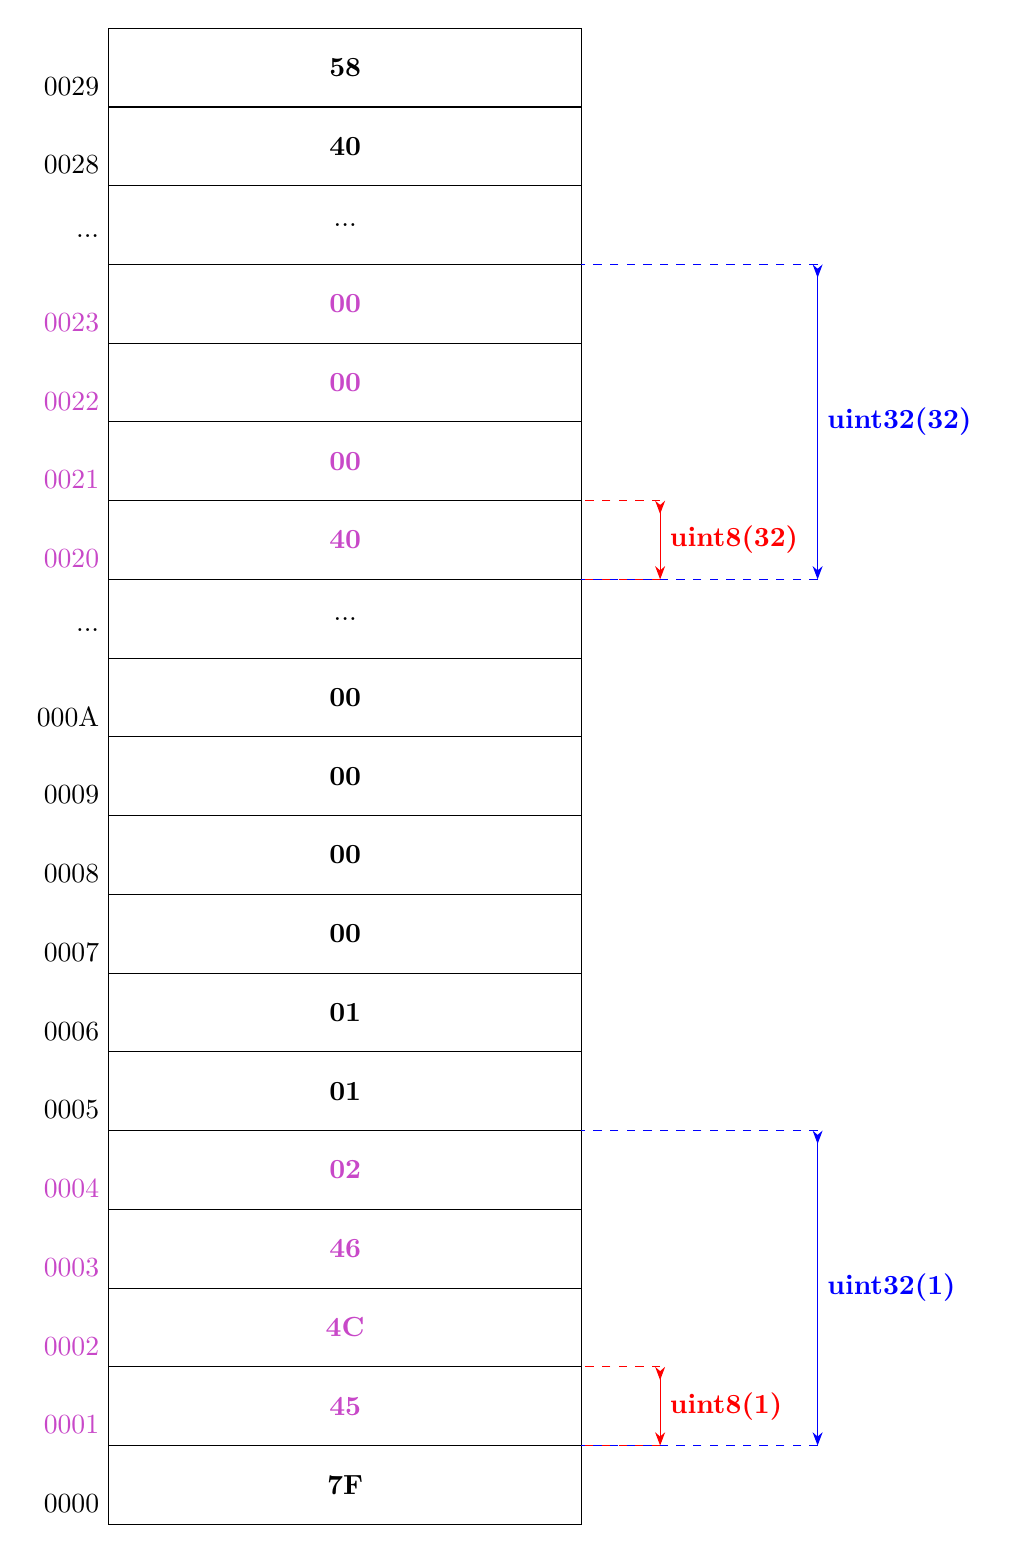
\begin{tikzpicture}[>=latex, node distance=1.5cm]

% \draw (0,1) rectangle node {0000} (5,2);
% \node[below left] at (0,1.5) {0000:0000};

\def\nodes{ 0029/58, 0028/40, ${...}$/${...}$, 0023/00, 0022/00, 0021/00, 0020/40, ${...}$/${...}$, 000A/00, 0009/00, 0008/00, 0007/00, 0006/01, 0005/01, 0004/02, 0003/46, 0002/4C, 0001/45, 0000/7F}

    Draw rectangles and labels
    \foreach [count=\i] \address/\data in \nodes {


        \ifnum\i>3
            \ifnum\i<8
                \definecolor{mynodecolor}{RGB}{ 200,72,200 } 

            \else
                \definecolor{mynodecolor}{RGB}{ 0,0,0 }

            \fi

        \else
                \definecolor{mynodecolor}{RGB}{ 0,0,0 }
                
        \fi

        \ifnum\i>14
            \ifnum\i<19
                
                \definecolor{mynodecolor}{RGB}{ 200,72,200 } 

            \else
                \definecolor{mynodecolor}{RGB}{ 0,0,0 }

            \fi

        % \else
        %         \definecolor{mynodecolor}{RGB}{0,0,0}
                
        \fi

        
            
        \draw (0,-\i) rectangle node [color=mynodecolor] {\textbf {\data} } (6,-\i+1);
        \node[below left, align=center, color=mynodecolor] at (0,-\i+0.5) {\address};
            
    }

    \draw[<-<, >=Stealth,blue, anchor= center] (9,-18) -- node[right] {\textbf{uint32(1)}} (9,-14);
    \draw[<-<, >=Stealth,red, anchor= center] (7,-18) -- node[right] {\textbf{uint8(1)}} (7,-17);
    \draw[dashed, -, >=Stealth,red, anchor= center] (7,-17) -- node[right] {} (6,-17);
    \draw[dashed, -, >=Stealth,red, anchor= center] (7,-18) -- node[right] {} (6,-18);
    \draw[dashed, -, >=Stealth,blue, anchor= center] (9,-14) -- node[right] {} (6,-14);
    \draw[dashed, -, >=Stealth,blue, anchor= center] (9,-18) -- node[right] {} (6,-18);

    \draw[<-<, >=Stealth,blue, anchor= center] (9,-7) -- node[right] {\textbf{uint32(32)}} (9,-3);
    \draw[<-<, >=Stealth,red, anchor= center] (7,-7) -- node[right] {\textbf{uint8(32)}} (7,-6);
    \draw[dashed, -, >=Stealth,red, anchor= center] (7,-7) -- node[right] {} (6,-7);
    \draw[dashed, -, >=Stealth,red, anchor= center] (7,-6) -- node[right] {} (6,-6);
    \draw[dashed, -, >=Stealth,blue, anchor= center] (9,-3) -- node[right] {} (6,-3);
    \draw[dashed, -, >=Stealth,blue, anchor= center] (9,-7) -- node[right] {} (6,-7);


\end{tikzpicture}



%\end{document}

\begin{itemize}

    
    \item \textbf{uint8(x)} prints the byte that is located at the decimal position x, counted through a zero based indexing. The first byte from the the starting is at 0, second one is at 1 and so on.

     \item \textbf{uint32(x)} prints the word that is located at the start of decimal position x, counted through a zero based indexing. The word is located in order $x+3 \rightarrow x+2 \rightarrow x+1 \rightarrow x$ The word from the the starting is at order $3 \rightarrow 2 \rightarrow 1 \rightarrow 0$, second one is at $4 \rightarrow 3 \rightarrow 2 \rightarrow 1$ and so on.

     \item \textbf{filesize} prints the size of the file in bytes. The libxselinux.so file is of 24512 bytes.

     
\end{itemize}

\begin{figure}[H]

    \centering
    \includegraphics[width=\textwidth]{hex_file.png}
    \caption{Detecting position from hex file}
    \label{fig:file_hex}
    
\end{figure}

\section{Conclusion}

YARA rules are syntactically flexible and the architecture is also modular with a robust framework. With its extensive community support, YARA continues to evolve as a vital asset in the arsenal of cybersecurity professionals, enabling proactive defense measures against emerging threats and facilitating collaborative efforts in the fight against cybercrime.


\end{document}
